

Nach dem Start der Anwendung wird der Benutzer direkt zum Anmeldebildschirm weitergeleitet. Dort kann sich ein bestehender Nutzer mit seinem Benutzernamen und Passwort anmelden. Alternativ kann über den Link \glqq Registrierung\grqq{} ein neuer Account erstellt werden.

\begin{figure}[H]
    \centering
    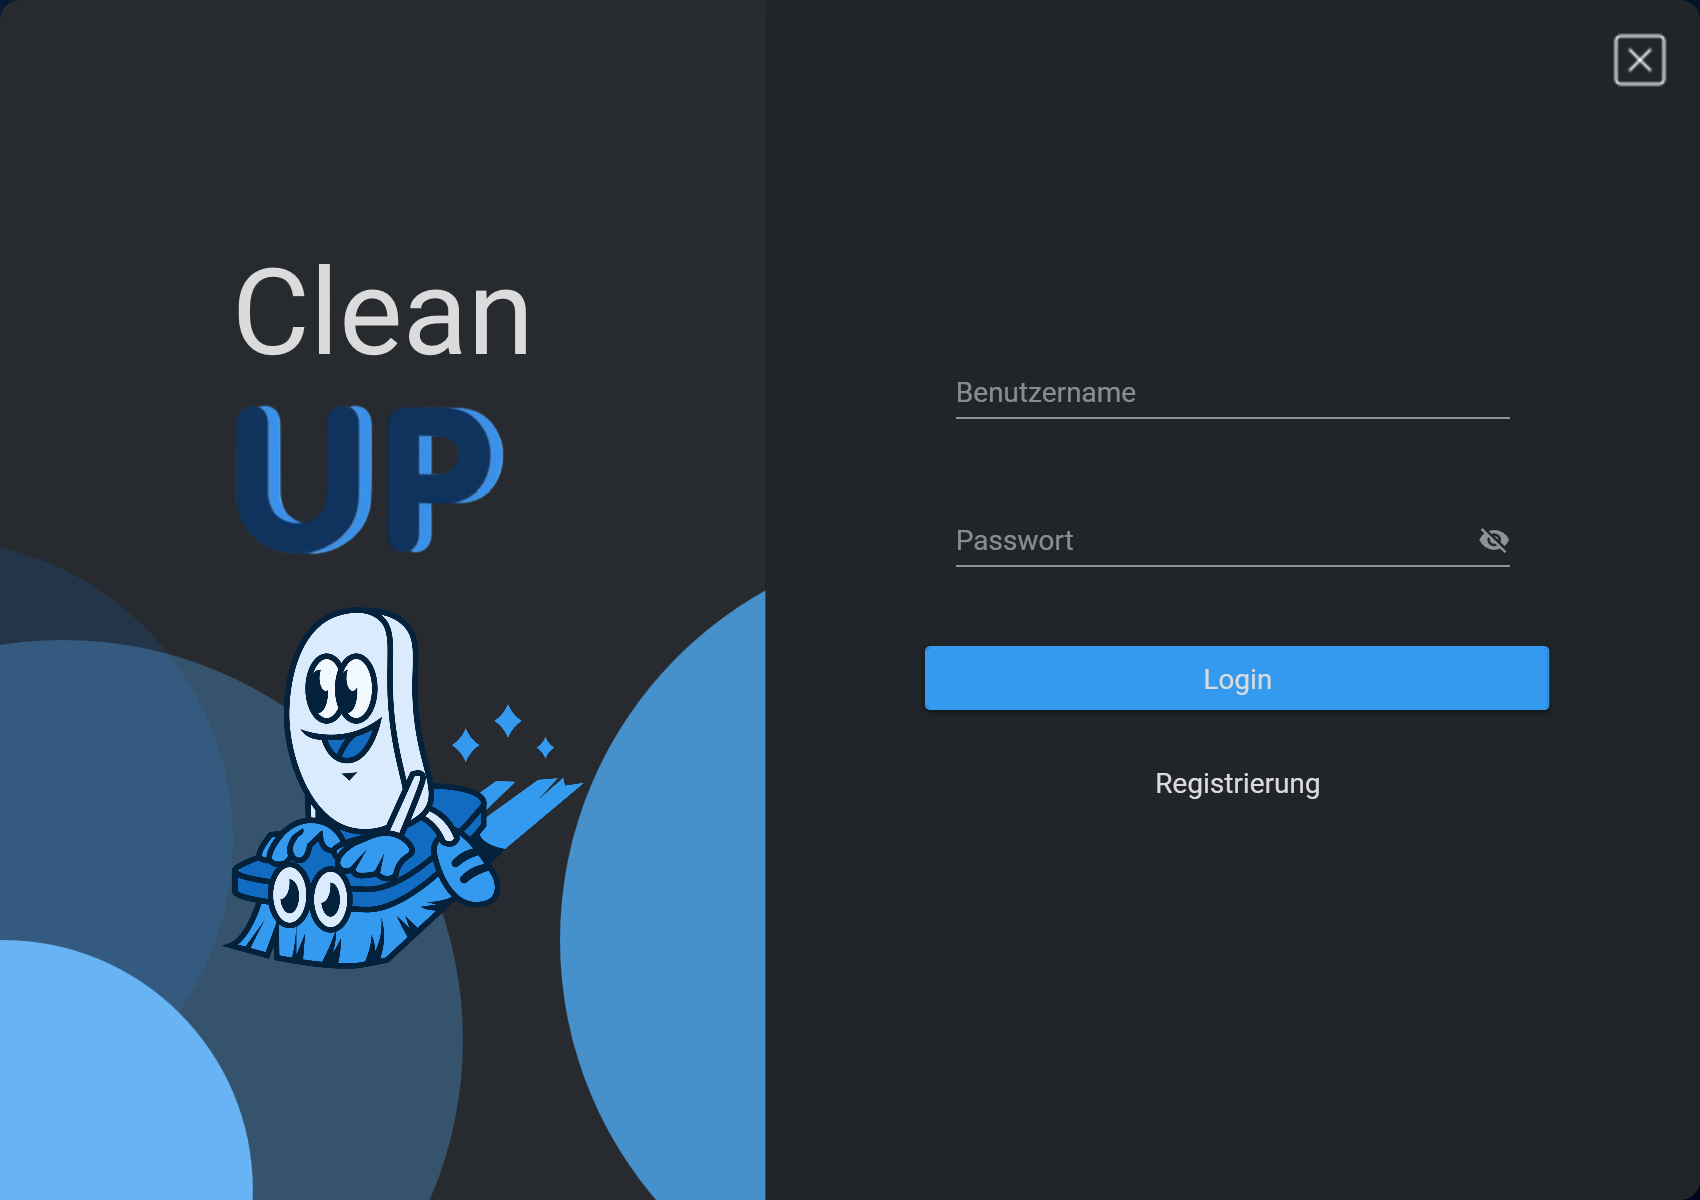
\includegraphics[width=0.8\textwidth]{src/screenshot_login.png}
    \caption{Login-Maske mit Eingabefeldern für Benutzername und Passwort}
\end{figure}

Bei der Registrierung müssen ein Benutzername sowie ein sicheres Passwort (mindestens 8 Zeichen) eingegeben und bestätigt werden. Das System überprüft die Eingaben und gibt bei fehlerhafter Eingabe eine visuelle Rückmeldung. Nach erfolgreicher Registrierung wird eine grüne Bestätigung angezeigt. Der Benutzer kann anschließend über den Link \glqq Zurück zum Login\grqq{} zum Anmeldebildschirm zurückkehren und sich mit den zuvor gewählten Anmeldedaten einloggen.

\begin{figure}[H]
    \centering
    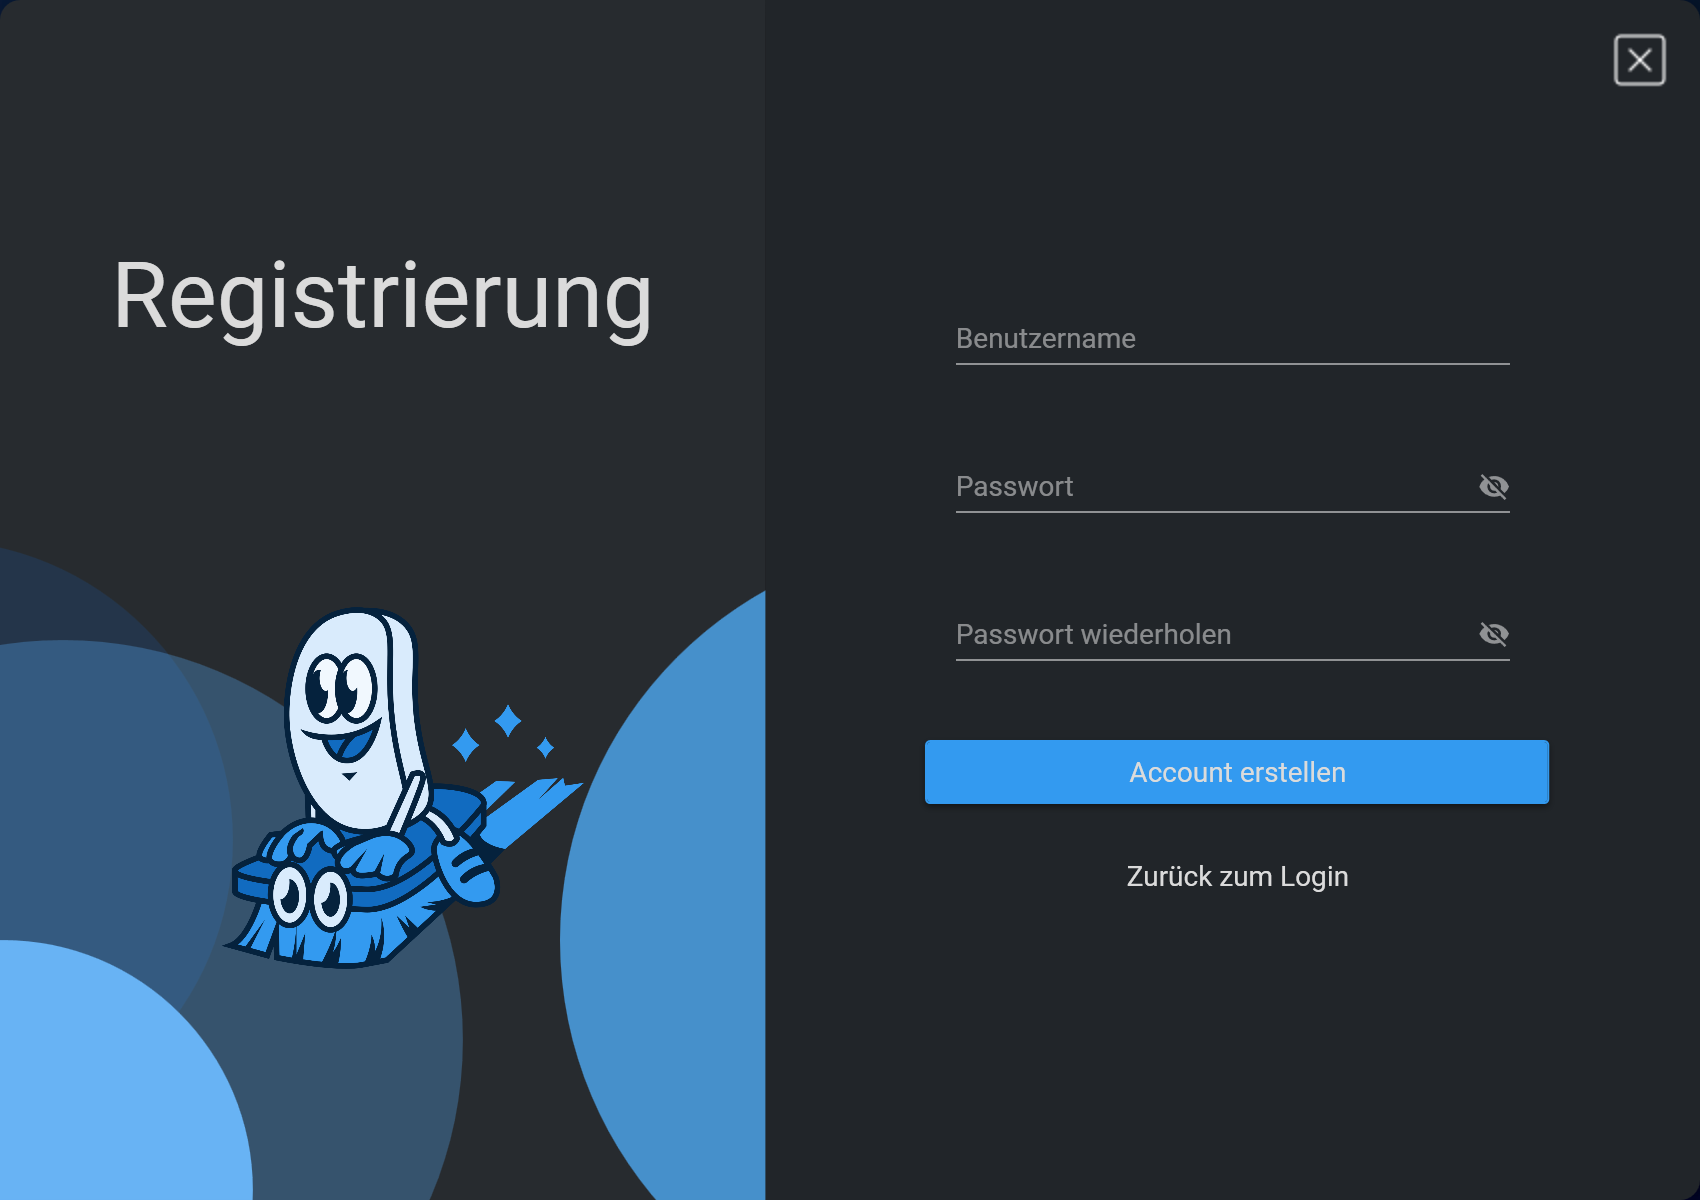
\includegraphics[width=0.8\textwidth]{src/screenshot_register.png}
    \caption{Registrierungsformular mit Passwortbestätigung}
\end{figure}

Nach erfolgreicher Anmeldung wird der Benutzer auf den Home-Bildschirm der Anwendung weitergeleitet und dort mit einer persönlichen Willkommensnachricht begrüßt. Zusätzlich werden ihm Statistiken zur Anwendung angezeigt, darunter die Gesamtanzahl gelöschter Dateien, der freigegebene Speicherplatz sowie eine Historie der letzten fünf durchgeführten Bereinigungsvorgänge. 

Bei Bedarf kann der Nutzer seine gesamte Historie einsehen, indem er seine Statistiken über den Button \glqq Logs exportieren\grqq{} als \texttt{.csv}-Datei herunterlädt. Auf Wunsch können die Statistiken auch vollständig zurückgesetzt und gelöscht werden. 

Über das Menü, welches als Sidebar umgesetzt wurde, kann der Nutzer nach Belieben zwischen den einzelnen Ansichten hin- und herwechseln.

\begin{figure}[H]
    \centering
    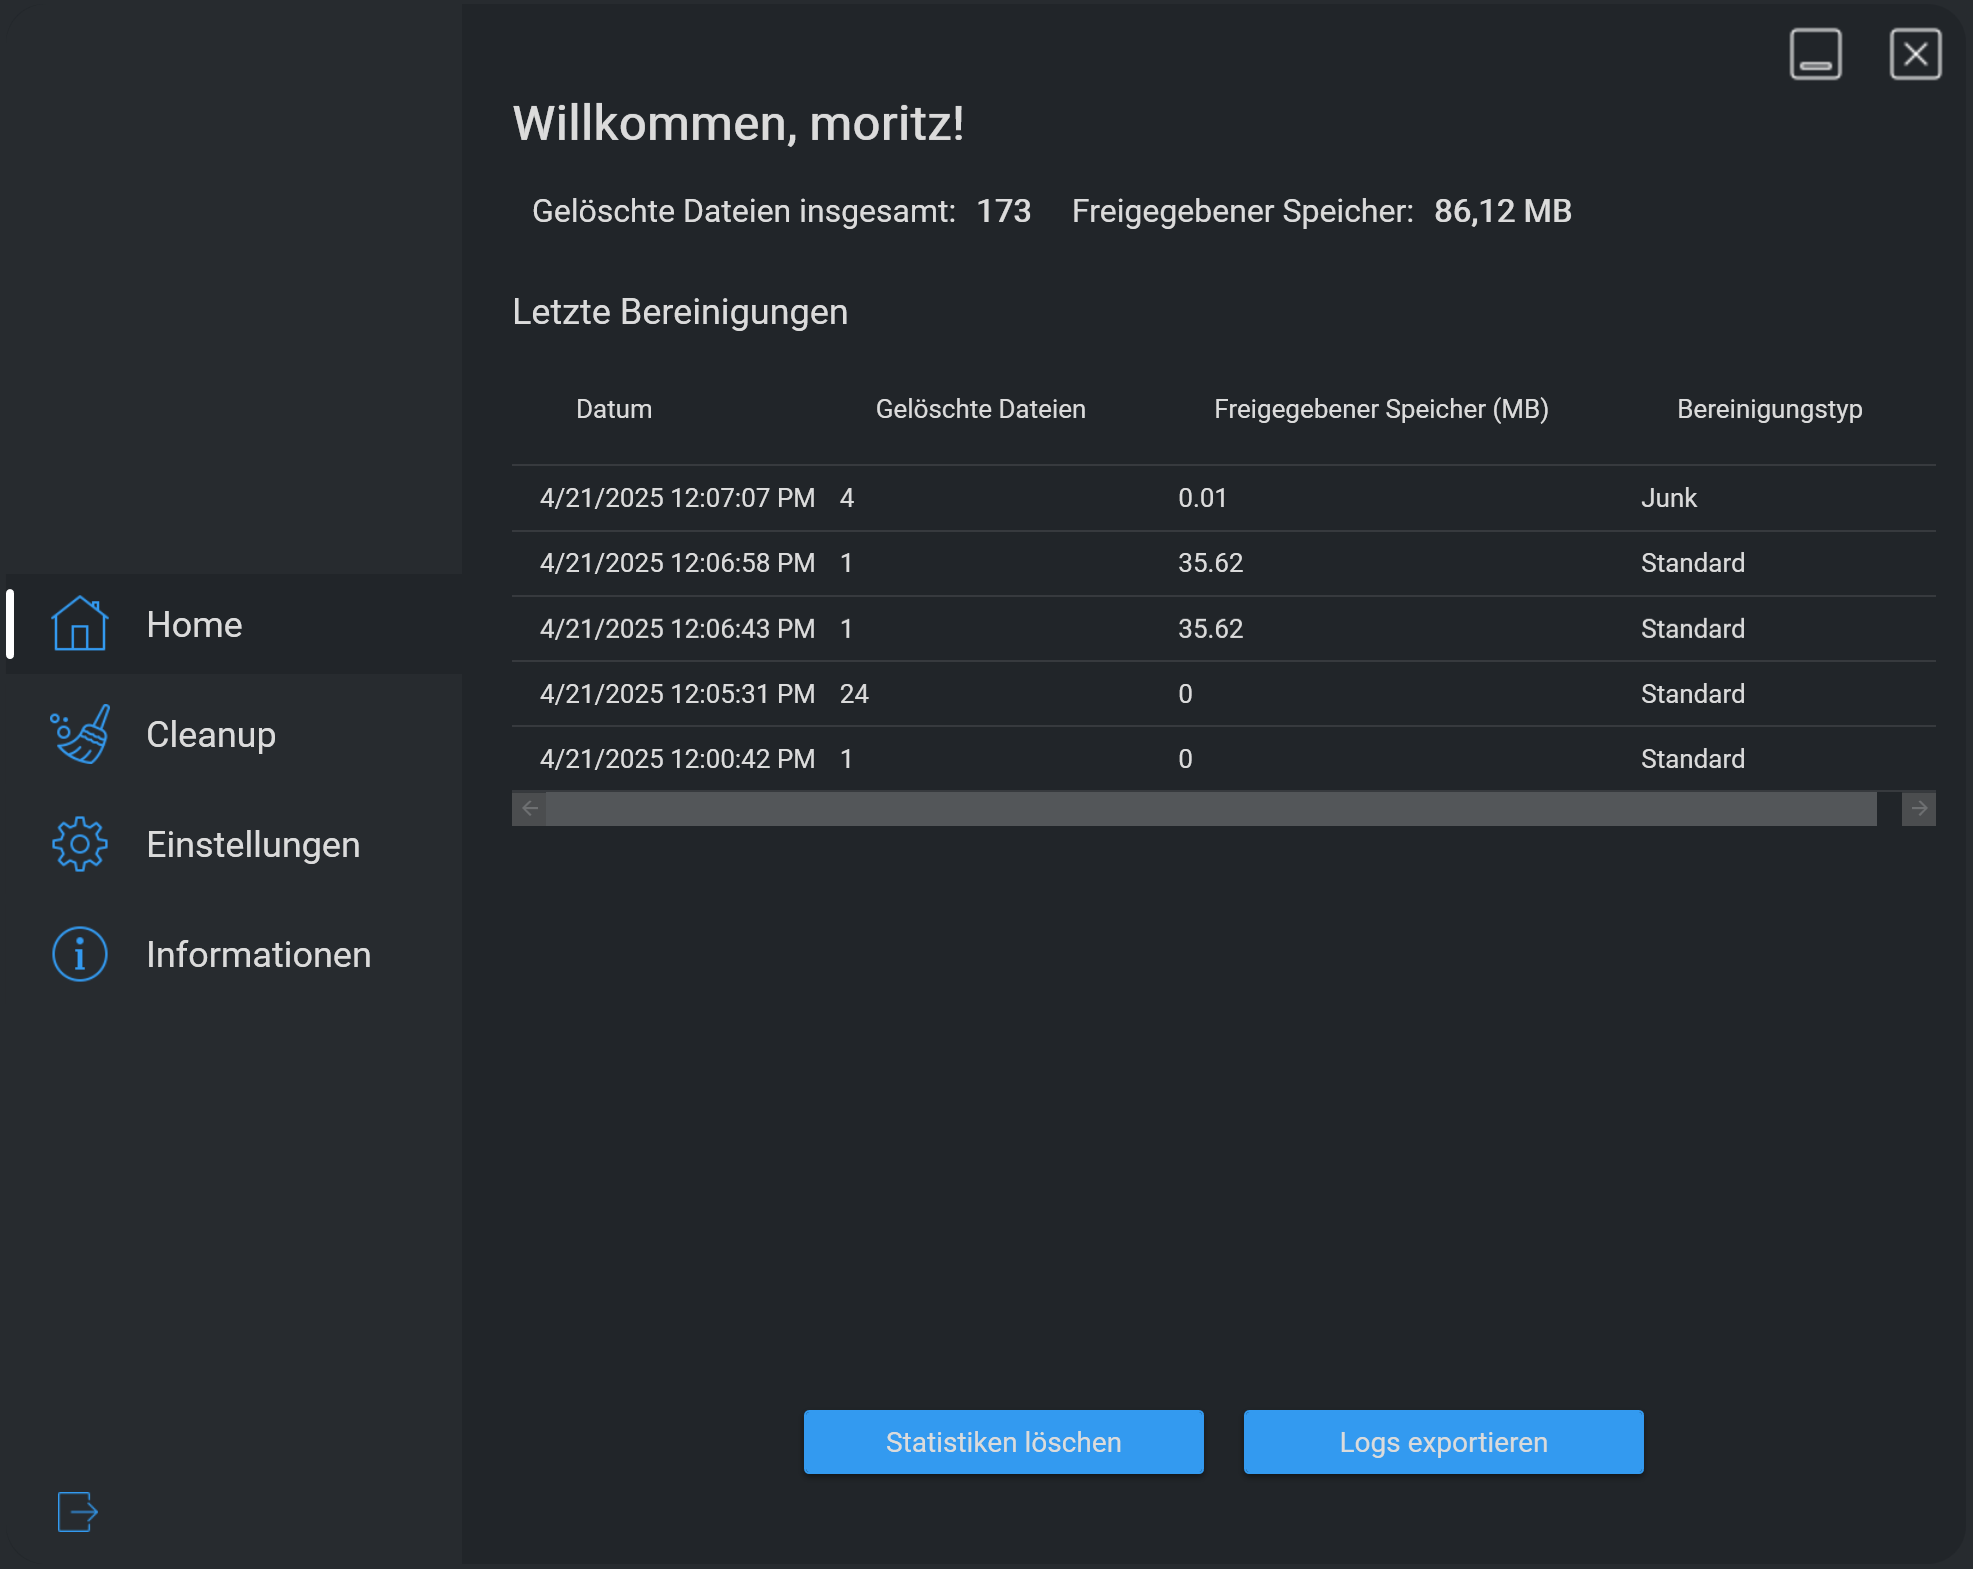
\includegraphics[width=0.9\textwidth]{src/screenshot_home.png}
    \caption{Home-Bildschirm des Nutzers mit dem gesetzten Benutzernamen \glqq moritz\grqq{}}
\end{figure}

